\documentclass[10pt,twocolumn]{article}
\usepackage[margin=0.72in]{geometry}
\usepackage{times,amsmath,graphicx}
\setlength{\columnsep}{0.22in}
\setlength{\textfloatsep}{7pt plus 1pt minus 2pt}
\setlength{\floatsep}{6pt plus 1pt minus 2pt}
\setlength{\intextsep}{6pt plus 1pt minus 2pt}
\newcommand{\dice}{\mathrm{Dice}}
\title{Response-Gated Background Prompting for Reference-Guided Nuclei Segmentation}
\author{Anonymous Authors\\Paper under double-blind review}
\date{}
\begin{document}
\maketitle

\begin{abstract}
Reference-guided segmentation can adapt a frozen foundation segmenter from one annotated support image, but a fixed prompt policy cannot decide whether background constraints help a particular query. We introduce a response-gated background prompting rule for dense nuclei segmentation. A frozen DINOv2 matcher builds foreground--background contrast prompts from a reference mask. A train-only gate then compares a default and a five-negative-point challenger using only observable SAM response changes, and falls back to the default when the challenger is not predicted to help. On 37 MoNuSeg cases under five-fold nested cross-validation, foreground--background matching improves Dice by $0.0647$ over foreground-only matching. The gate further improves Dice over the fold-specific anchor by $0.0101$ (95\% CI $[0.0039,0.0188]$) and closes 66.1\% of the fixed-to-oracle gap. On a frozen 2,540-tile PanNuke field-level diagnostic, fixed N5 degrades N0, while the version-isolated five-fold gate improves N0 by $0.0047$ (95\% CI $[0.0040,0.0054]$). Patient-disjoint MoNuSAC and SAM-Med2D tests delimit the claim: response-aware prompting is useful but segmenter- and domain-conditioned rather than universal.
\end{abstract}

\noindent\textit{Index Terms---}medical image segmentation, foundation models, prompt engineering, selective decision, few-shot segmentation.

\section{Introduction}
Promptable segmentation models make it possible to define a task with a small number of points or a reference image-mask pair. Segment Anything (SAM)~\cite{kirillov2023sam} and feature backbones such as DINOv2~\cite{oquab2024dinov2} have enabled reference-guided medical segmentation, including one-shot automatic prompting~\cite{liu2025sat}. Yet, the points passed to the frozen segmenter are commonly selected by a fixed rule. This is problematic for dense all-nuclei segmentation: background points can suppress false-positive connections in one patch and erase true nuclei in another.

Recent background-centric prompting work, notably FoB~\cite{bo2026fob}, confirms that support-background localization is important for few-shot medical segmentation. Our question is narrower and complementary: once reference foreground--background evidence fixes a positive prompt set, \emph{when should the observable response to an additional background constraint be accepted?} Answering this question with a small, auditable action space avoids claiming that any one prompt policy is universal across domains or segmenters.

Our contributions are: (i) a foreground--background contrast representation that substantially improves reference-defined point placement; (ii) a two-candidate response gate that predicts whether a five-point background challenger should replace a validation-selected anchor; and (iii) nested, patient-disjoint, and frozen field-level analyses that report both positive results and domain/segmenter failure boundaries.

\section{Method}
\subsection{Foreground--background contrast prompts}
For reference image $R$, binary mask $M_R$, and query image $Q$, frozen DINOv2 features yield normalized reference prototypes $p_{fg}$ and $p_{bg}$ by averaging feature tokens inside and outside $M_R$. For a query token $x$, we form
\begin{equation}
s(x)=z(\cos(F_Q(x),p_{fg}))-0.75z(\cos(F_Q(x),p_{bg})).
\end{equation}
The 40 highest-scoring patch centers form the shared positive set. This foreground--background contrast explicitly treats the support mask complement as evidence rather than assuming it is uninformative.

\subsection{Response-gated background budget}
We use the candidate action set $\mathcal{A}=\{N0,N5\}$, where $N$ is the requested number of spatially separated background points sampled from low contrast-score positions. Within each outer training fold, inner validation selects a fixed anchor $a_0$. A pre-SAM ExtraTrees regressor chooses the alternative challenger, while retaining $a_0$. SAM receives both prompts with a shared image embedding. A second train-only ExtraTrees regressor predicts the challenger's gain using deployment-available differences in SAM mask-quality score, predicted foreground area, and actual negative-point count. The output is
\begin{equation}
\hat{Y}=\begin{cases}S(Q,a_c),&\widehat{\Delta\dice}(a_c,a_0)>\tau,\\S(Q,a_0),&\text{otherwise},\end{cases}
\end{equation}
where $\tau$ is selected on inner validation. Ground truth is used only to construct training rewards and evaluate held-out cases. Thus the gate is a constrained response-selection rule, not a differentiable SAM fine-tuning method.

\section{Experimental protocol}
MoNuSeg~\cite{kumar2019monuseg} provides the primary dense-nuclei experiment. We use five-fold nested CV on its 37 source-train cases: 37 independent outer-test queries, five inner-train references per query, and 185 reference episodes. The 14 official test cases are excluded from model selection. We average the five reference outcomes per query before paired inference; 95\% CIs use 10,000 paired bootstrap resamples (seed 20260715).

For external transfer, MoNuSAC~\cite{verma2021monusac} uses patient-disjoint train/validation/test partitions of 154/46/101 patches from 35/9/25 patients. Support and query never share a patient. We report both patch and patient aggregates. A 128-pair CPU/GPU audit produced identical coordinates and maximum Dice difference 0.000145, below its predeclared 0.0002 tolerance.

Before downloading PanNuke, we froze a field-level zero-shot diagnostic: every nonempty fold-1 tile (2,540) is queried with five hash-selected nonempty fold-2 supports; the five outcomes are averaged before paired bootstrap. No patient identifiers are available in the public release, so this is not a patient-disjoint analysis. The DINOv2-L and SAM ViT-B inference path is unchanged. Raw N0/N5 outputs are generated before any gate loading; folds 0--1 (sklearn 1.7.2) and folds 2--4 (sklearn 1.9.0) are separately deserialized, then deterministically majority-voted. The gate consumes SAM score/area response changes and fixed action differences, never PanNuke Dice or masks.

\section{Results and analysis}
\begin{table}[t]
\caption{Evidence-locked results. CIs are paired 95\% bootstrap CIs. MoNuSAC N5 is post-hoc and is not a model-selection baseline.}
\centering\scriptsize
\begin{tabular}{lccc}
\hline
Comparison & $n$ & $\Delta\dice$ & 95\% CI\\
\hline
FG-BG N0 vs. FG-only (MoNuSeg) & 37 & +.0647 & [.0470,.0841]\\
Gate vs. fold anchor (MoNuSeg) & 37 & +.0101 & [.0039,.0188]\\
Gate vs. fixed N5 (MoNuSeg) & 37 & +.0092 & [.0004,.0193]\\
Frozen gate vs. N0 (MoNuSAC) & 101 & +.0079 & [.0016,.0155]\\
Frozen gate vs. N0 (MoNuSAC patients) & 25 & +.0076 & [.0018,.0146]\\
Fixed N5 vs. N0 (PanNuke) & 2540 & -.0127 & [-.0143,-.0112]\\
Five-fold gate vs. N0 (PanNuke) & 2540 & +.0047 & [.0040,.0054]\\
Gate vs. anchor (Med2D) & 37 & -.0003 & [-.0009,.0000]\\
\hline
\end{tabular}
\label{tab:effects}
\end{table}

Foreground--background contrast is the dominant mechanism: it raises mean MoNuSeg Dice from 0.4733 to 0.5380, winning 36 of 37 cases (Table~\ref{tab:effects}). With this shared prompt representation, the learned gate achieves 0.5476 Dice, versus 0.5375 for the fold anchor and 0.5384 for globally fixed N5. It switches only where predicted response gain is positive; its per-query oracle is 0.5523, so the gate closes 66.1\% of the global-N5-to-oracle gap. Figure~\ref{fig:main} aggregates the primary effects. A diagnostic component analysis does not show a clear object-level gain (object-recall $\Delta=-.0022$, 95\% CI $[-.0056,.0000]$; merge-error $\Delta=+.0027$, $[-.0002,.0056]$), so our positive claim is deliberately limited to union-mask Dice rather than instance separation.

\begin{figure}[t]
\centering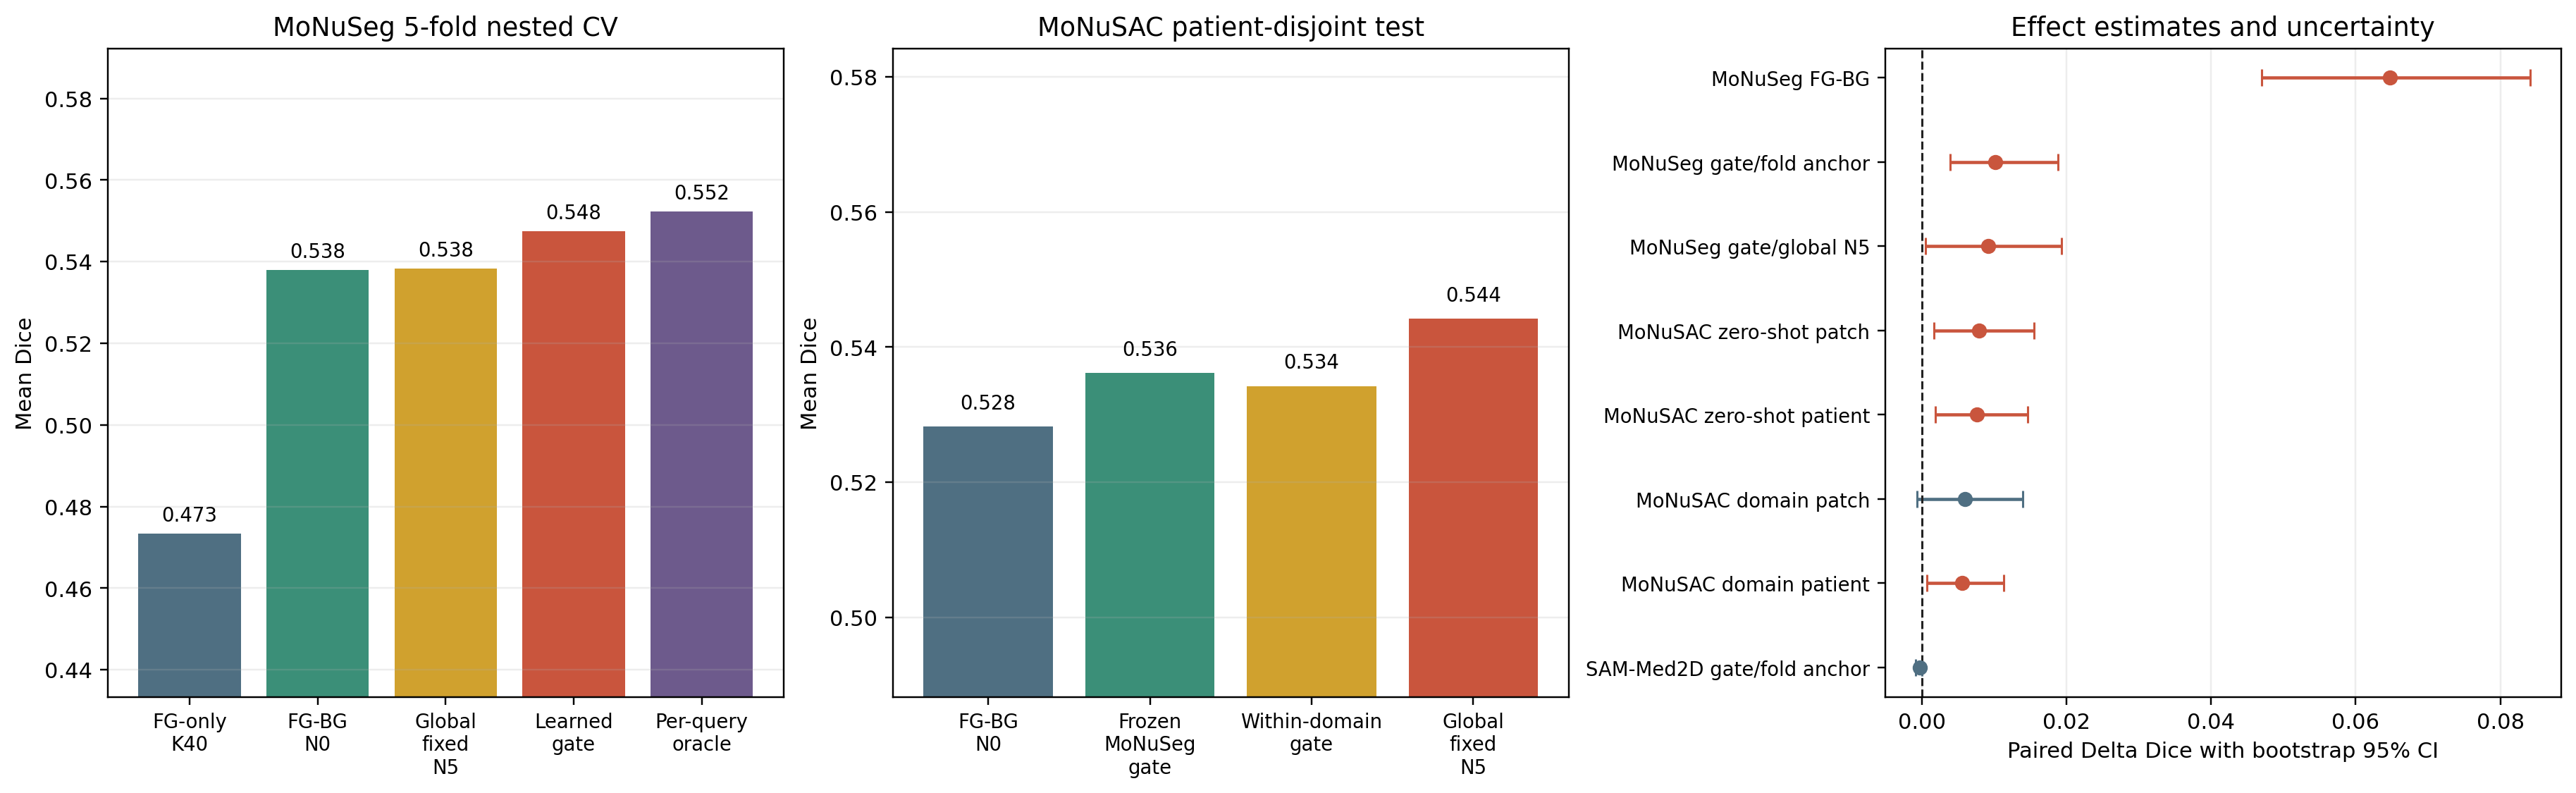
\includegraphics[width=\columnwidth]{figures/main_results.png}
\caption{Primary nested-CV effects and the patient-disjoint MoNuSAC boundary.}
\label{fig:main}
\end{figure}

The patient-disjoint MoNuSAC transfer supports a limited conclusion: the frozen MoNuSeg gate improves N0 from 0.5283 to 0.5362. After patch and reference averaging, the patient-level mean also improves from 0.5350 to 0.5426 ($\Delta=+.0076$, bootstrap 95\% CI $[+.0018,+.0146]$; 14/5/6 win/tie/loss). Its two-sided patient sign test is $p=.115$, so this is directional corroboration rather than a standalone rank-test confirmation. It does not exceed the observed post-hoc global N5 mean of 0.5442. Similarly, a protocol-matched SAM-Med2D experiment has a non-positive gate effect. These outcomes are important: they reject model-agnostic and domain-optimal interpretations. Qualitative examples (Fig.~\ref{fig:qual}) show the intended gain (removing broad false positives) and a failure case (over-suppressing true nuclei).

The pre-registered PanNuke diagnostic supplies a complementary stress test. Fixed N5 falls from 0.4927 to 0.4800 Dice ($\Delta=-.0127$, 95\% CI $[-.0143,-.0112]$), whereas the frozen five-fold majority gate reaches 0.4974 ($\Delta$ vs. N0 $=+.0047$, 95\% CI $[+.0040,+.0054]$). It wins/ties/loses against N0 on 1,354/469/717 query tiles. In post-hoc descriptive breakdowns, the direction is retained for each of the five fixed supports (gate-vs-N0 CI lower bounds 0.0025--0.0044), while public tissue-code strata yield 15 positive, four indeterminate, and no negative gate CIs (17--816 tiles/stratum). No support or subgroup was selected from these analyses. This does not establish patient-level generalization or PanNuke tuning: it instead shows that a gate trained elsewhere can reject a systematically harmful fixed background policy in a large, held-out field-level cohort.

\paragraph{Latency.} On an NVIDIA GeForce RTX 5090 D v2, we timed 30 CUDA-synchronized 256$\times$256 PanNuke support--query episodes after five warmups, without opening a query annotation. The full DINOv2-L matching plus SAM ViT-B image embedding and N0/N5 dual-decode path has median/p90 latency 240.7/389.4 ms, including support/query reads and support/query DINO features. When the support representation is cached, its median/p90 is 178.9/309.3 ms. These are single-GPU inference measurements, not an end-to-end clinical-system throughput claim.

\paragraph{FoB transfer diagnostic.} We also adapted the released FoB implementation to frozen MoNuSeg fold 0: 1,000 train-only steps on 115 episodes, four pre-registered checkpoints, 30 inner-validation episodes for selection, and one 40-episode outer test. Its selected SAM ViT-H configuration obtained 0.0048 Dice. Query masks were read only after prompt generation and SAM decoding to calculate Dice. This is a negative transfer diagnostic, not a head-to-head result: it covers one fold and a different segmenter configuration from our five-fold DINOv2-L + SAM ViT-B protocol. It reinforces the need to report domain and implementation boundaries rather than claim superiority to FoB.

\begin{figure*}[t]
\centering
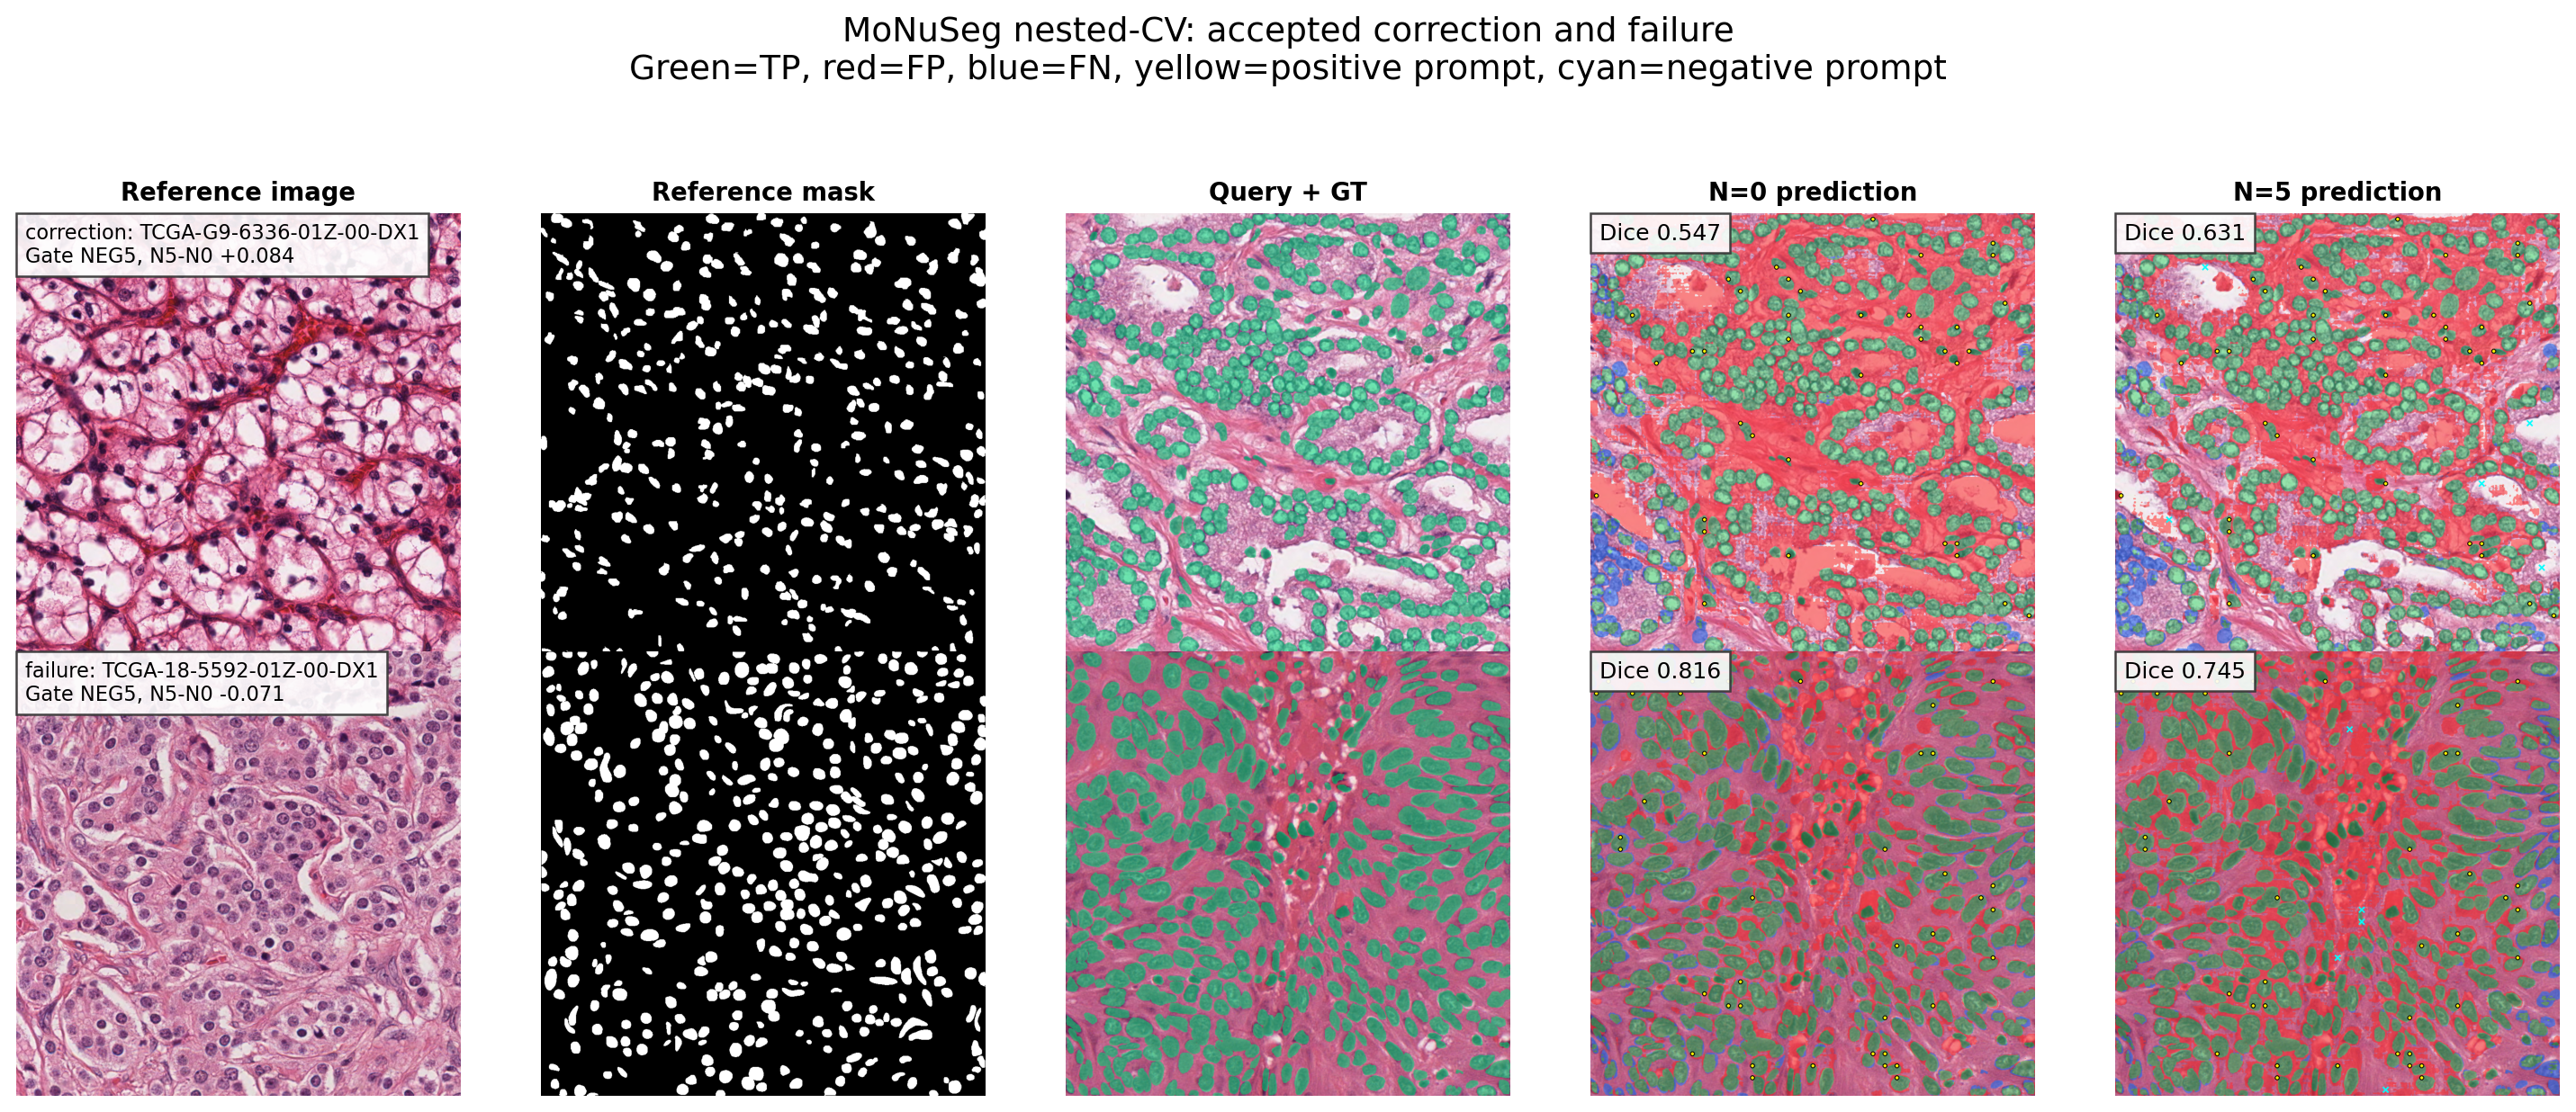
\includegraphics[width=.49\textwidth]{figures/monuseg_qualitative.png}\hfill
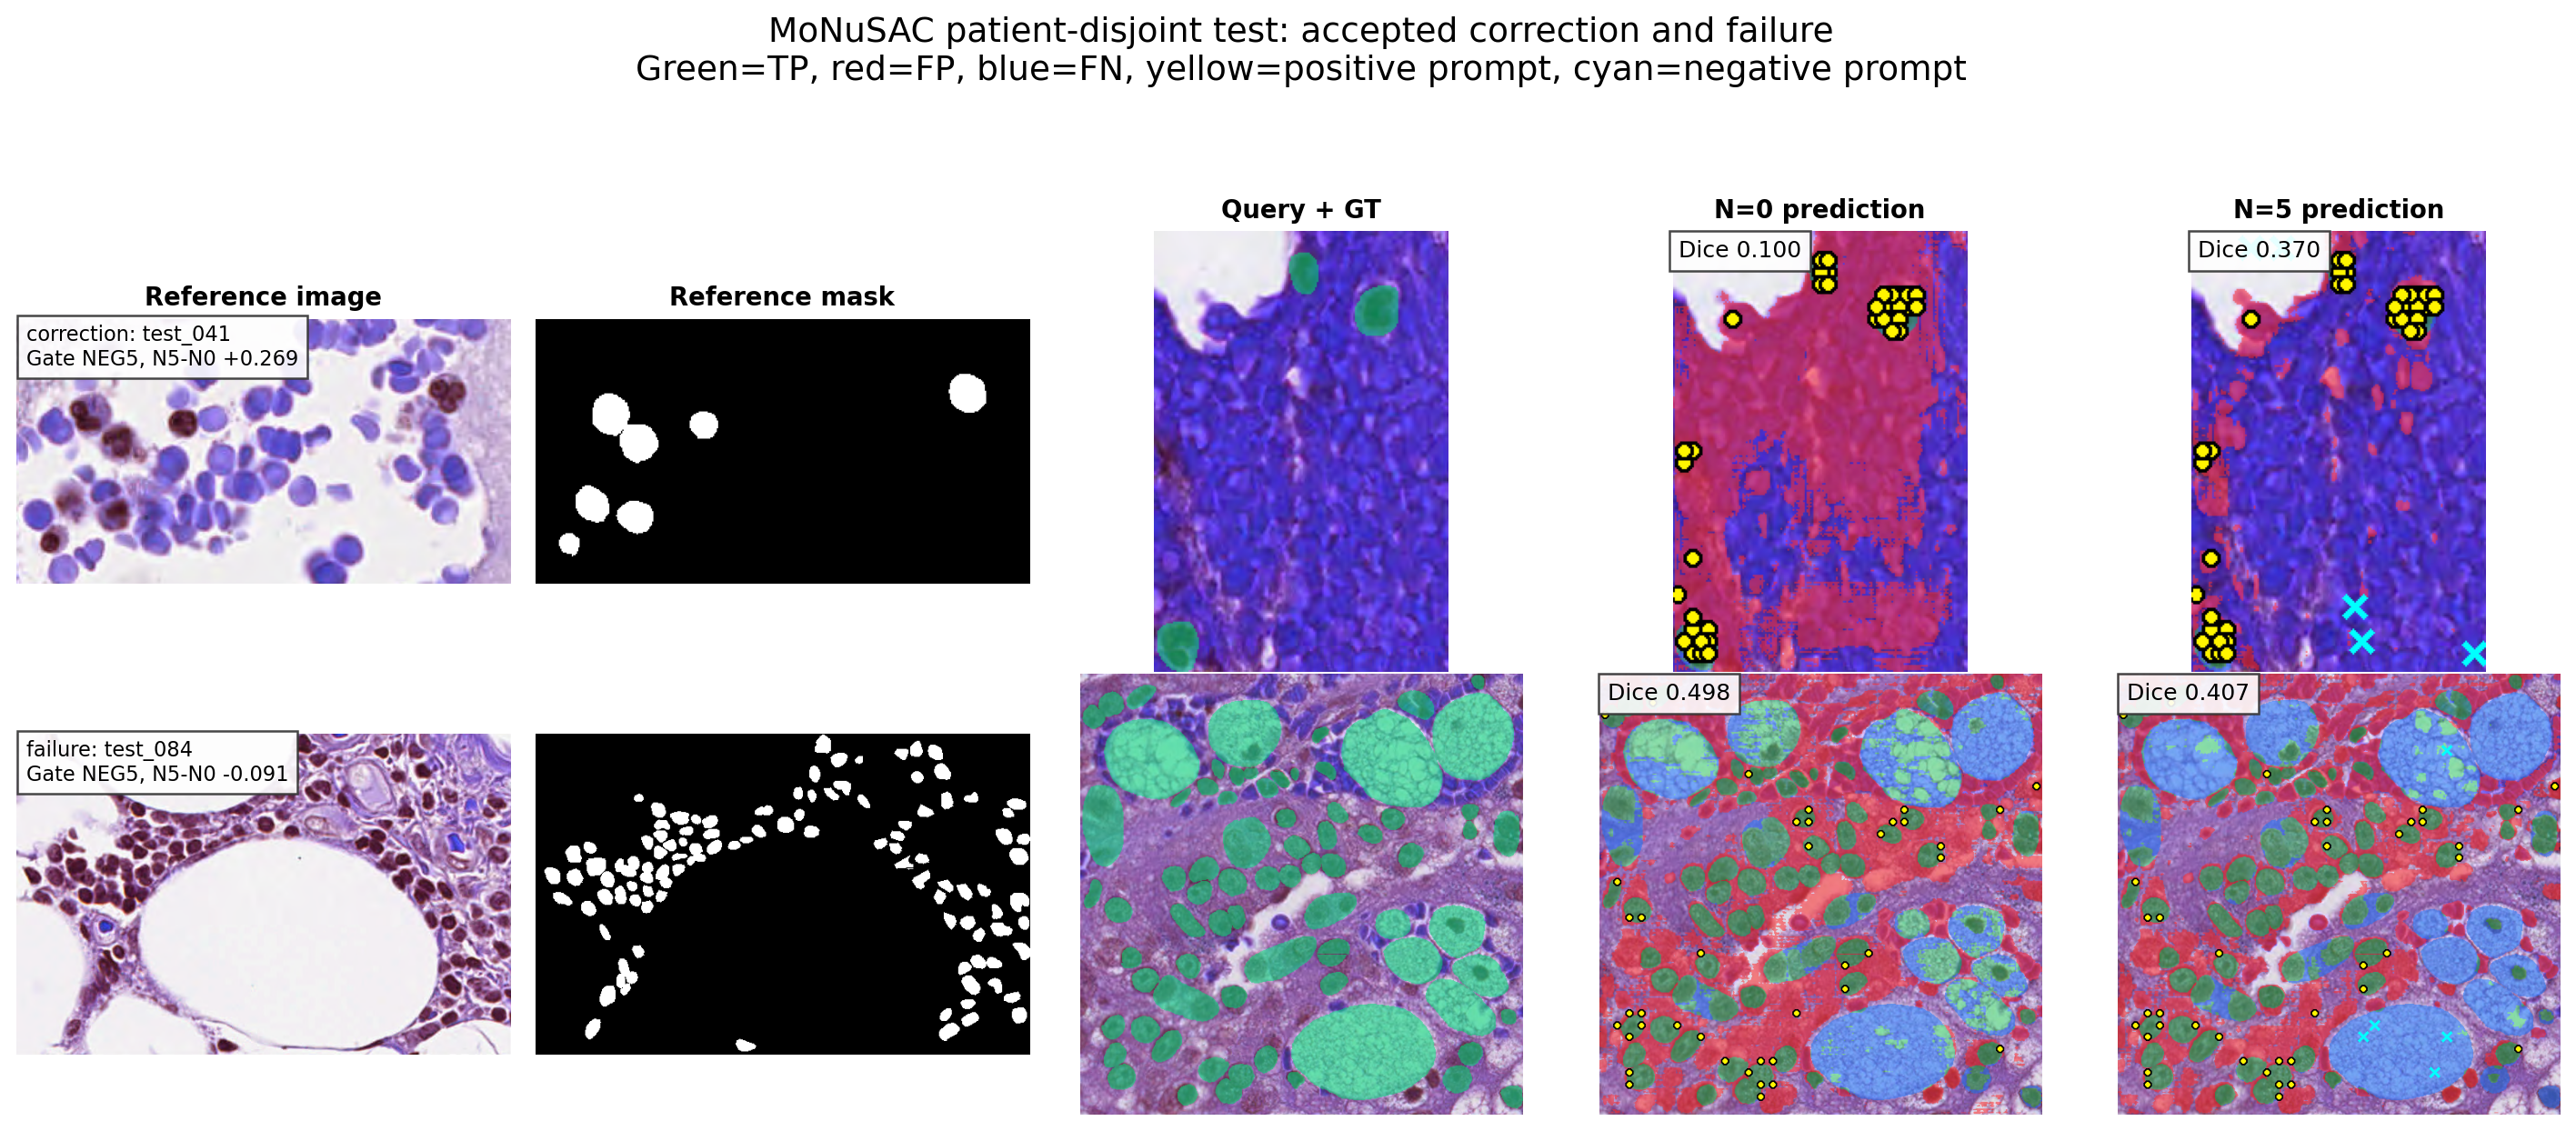
\includegraphics[width=.49\textwidth]{figures/monusac_qualitative.png}
\caption{Reference-aware qualitative evidence. Left: nested MoNuSeg success/failure examples. Right: patient-disjoint MoNuSAC examples. Green/red/blue indicate TP/FP/FN; yellow/cyan marks positive/negative prompts.}
\label{fig:qual}
\end{figure*}

\section{Conclusion}
Foreground--background reference evidence materially improves dense-nuclei prompt placement, and a constrained response gate yields statistically positive improvements for frozen DINOv2-L + SAM ViT-B in nested MoNuSeg and a pre-registered PanNuke field-level diagnostic. The patient-disjoint, cross-segmenter, and one-fold FoB-adaptation boundaries delimit the claim: response gating is not a universal prompt policy. The next necessary tests are a fully protocol-matched multi-fold comparator reproduction and a further patient-disjoint pathology cohort.

\newpage
\begin{thebibliography}{00}
\bibitem{kirillov2023sam} A. Kirillov \emph{et al.}, ``Segment Anything,'' in \emph{Proc. ICCV}, 2023.
\bibitem{oquab2024dinov2} M. Oquab \emph{et al.}, ``DINOv2: Learning Robust Visual Features without Supervision,'' \emph{TMLR}, 2024.
\bibitem{liu2025sat} X. Liu \emph{et al.}, ``Segment Any Tissue: One-shot Reference Guided Training-free Automatic Point Prompting for Medical Image Segmentation,'' \emph{Medical Image Analysis}, vol. 102, p. 103550, 2025.
\bibitem{bo2026fob} Y. Bo, Y. Zhu, P. Koniusz, and H. Zhang, ``Focus on Background: Exploring SAM's Potential in Few-shot Medical Image Segmentation with Background-centric Prompting,'' in \emph{Proc. CVPR}, pp. 30032--30041, 2026.
\bibitem{kumar2019monuseg} N. Kumar \emph{et al.}, ``A Multi-organ Nucleus Segmentation Challenge,'' \emph{IEEE TMI}, vol. 39, no. 5, pp. 1380--1391, 2019.
\bibitem{verma2021monusac} R. Verma \emph{et al.}, ``MoNuSAC2020: A Multi-organ Nuclei Segmentation and Classification Challenge,'' \emph{IEEE TMI}, 2021.
\end{thebibliography}
\end{document}
